\documentclass{beamer}
\usepackage{animate}  % Add this package for GIF support
\usepackage{tcolorbox} % Package pour les boîtes colorées

% Thème du beamer (modifiable selon tes préférences)
\usetheme{Frankfurt}

% Afficher les numéros de pages en bas de chaque slide
\setbeamertemplate{footline}[frame number]

% Informations sur le document
\title{Cours de Vision par Ordinateur}
\author{Florian Valade}
\date{\today}

\begin{document}

% Page de titre
\begin{frame}
    \titlepage
\end{frame}

% Présentation de l'intervenant
\begin{frame}
    \frametitle{Présentation}
    \textbf{Florian Valade} \newline
    \href{mailto:florian.valade@univ-eiffel.fr}{florian.valade@univ-eiffel.fr} \newline
    Data Scientist chez Fujitsu \newline
    Chercheur au LAMA \newline
    \begin{columns}
        \begin{column}{0.5\textwidth}
            \begin{flushleft}
                
\includegraphics[width=0.3\textwidth]{images/lama.png}
            \end{flushleft}
        \end{column}
        \begin{column}{0.5\textwidth}
            \begin{flushright}
                
\includegraphics[width=0.3\textwidth]{images/fujitsu.png}
            \end{flushright}
        \end{column}
    \end{columns}
\end{frame}

% Section Introduction
\section{Introduction}

% Objectif du cours
\begin{frame}
    \frametitle{Objectif du cours}
    Comprendre la vision par ordinateur et ses applications industrielles \newline
    Permettre aux étudiants d'évoluer en tant que :
    \begin{itemize}
        \item Data Scientist
        \item Machine Learning Engineer
        \item Chercheur en Computer Vision
    \end{itemize}
\end{frame}

% Structure du cours
 \begin{frame}
    \frametitle{Structure du cours}
    \begin{itemize}
        \item \textbf{Introduction} : Fondamentaux du traitement d'images
        \begin{itemize}
            \item Représentation numérique des images
            \item Concepts clés en vision par ordinateur
        \end{itemize}
        \item \textbf{Méthodes classiques}
        \begin{itemize}
            \item Filtres et convolutions
            \item Détection de contours et segmentation
            \item Travaux pratiques sur des cas réels
        \end{itemize}
        \item \textbf{Deep Learning en Vision}
        \begin{itemize}
            \item Réseaux de neurones convolutifs (CNN)
            \item Architecture Transformer
            \item Applications modernes
        \end{itemize}
    \end{itemize}
\end{frame}

% Notation du cours
\begin{frame}
    \frametitle{Notation du cours}
    \textbf{Évaluation par projet}
    \begin{itemize}
        \item \textbf{Projet de Computer Vision} (100\% de la note finale)
        \begin{itemize}
            \item Développement d'une solution complète de vision par ordinateur
            \item Application des concepts vus en cours sur un cas concret
            \item Travail en groupe de 3-4 étudiants
        \end{itemize}
        \item \textbf{Livrables attendus}
        \begin{itemize}
            \item Code source documenté
            \item Rapport technique détaillé
        \end{itemize}
        \item \textbf{Date de rendu} : Fin du semestre
    \end{itemize}
\end{frame}

% Pourquoi la vision par ordinateur ?
\begin{frame}
    \frametitle{Pourquoi la vision par ordinateur ?}
    \textbf{Relier deux mondes :}
    \begin{itemize}
        \item Monde numérique : automatisation et manipulation aisée des données
        \item Monde physique : complexité de compréhension et d'automatisation
    \end{itemize}
\end{frame}

\begin{frame}
    \frametitle{Impact et Applications de la Vision par Ordinateur}
    \textbf{Permet d'étudier et d'influencer le monde physique}
    \begin{itemize}
        \item Détection de plants malades dans un champ
        \item Conduite autonome
        \item Robotique
        \item Surveillance industrielle 
        \item Reconnaissance faciale
        \item Détection d'objets en temps réel
    \end{itemize}
    \begin{center}
        \includegraphics[width=0.3\textwidth]{images/conduite_autonome.png}
        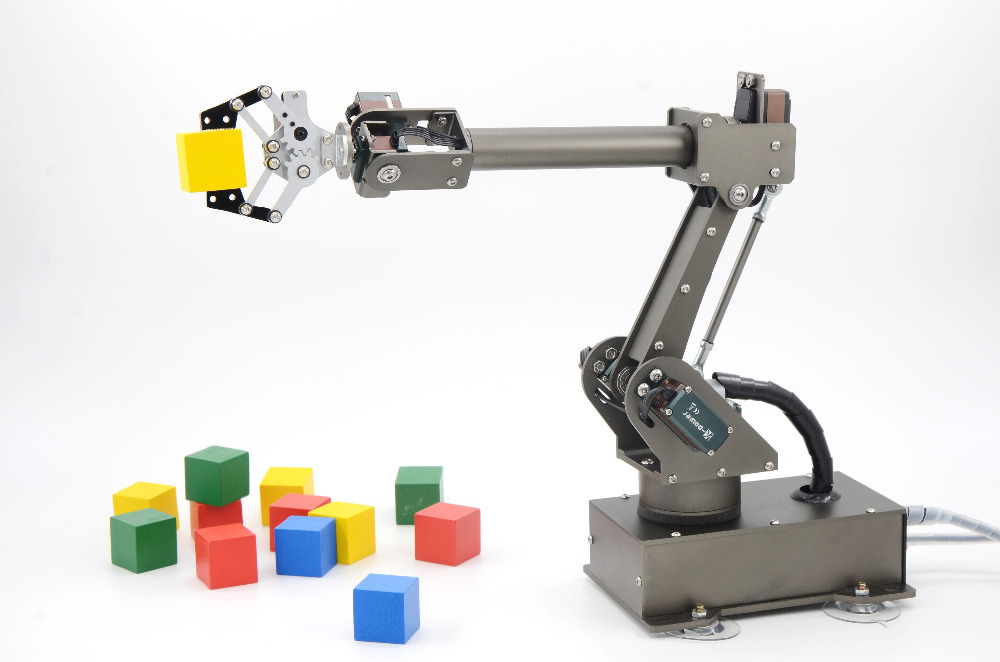
\includegraphics[width=0.3\textwidth]{images/robotique.png}
        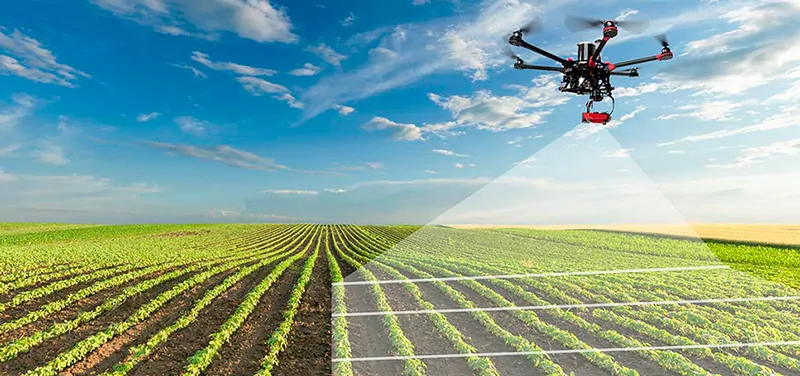
\includegraphics[width=0.3\textwidth]{images/detection_champ.png}
    \end{center}
\end{frame}

\begin{frame}
    \frametitle{Exemple Concret: Reconnaissance de Fruits et Légumes}
    \begin{columns}
        \column{0.5\textwidth}
        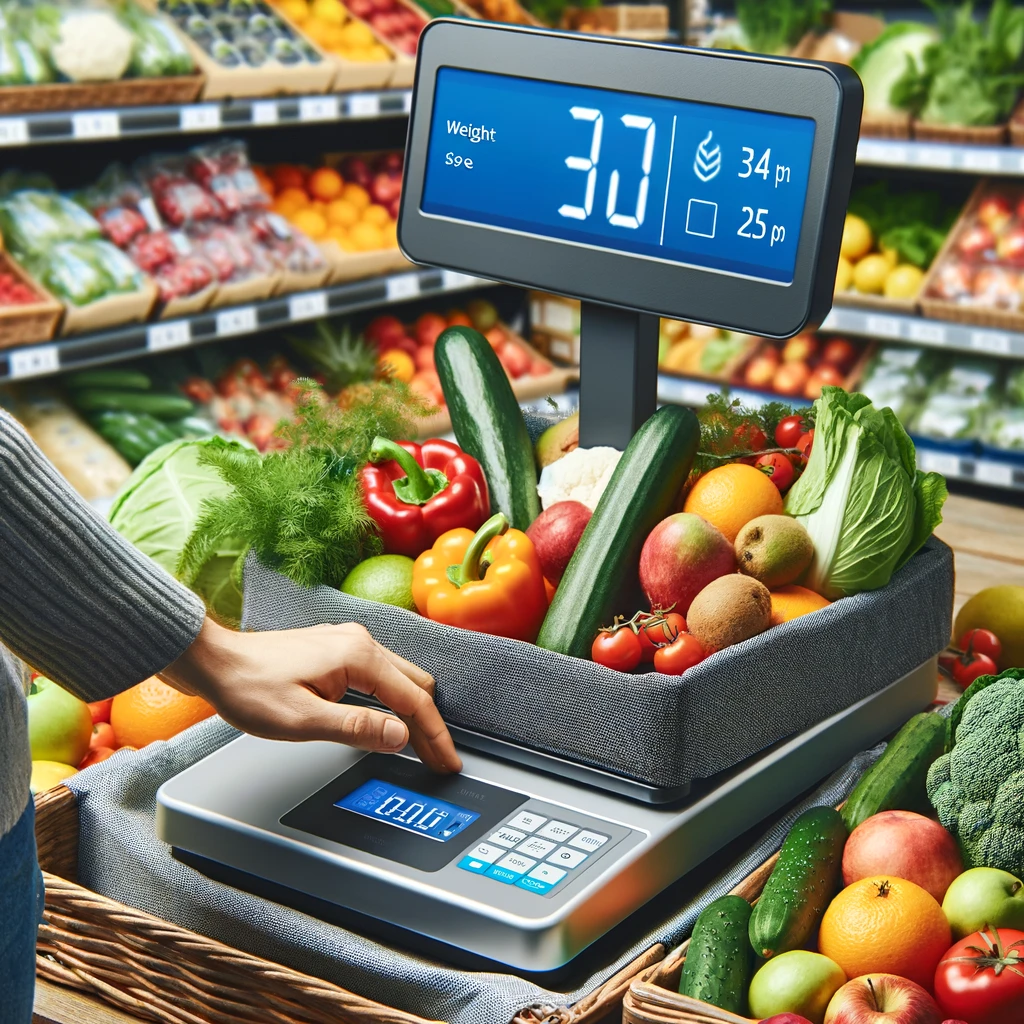
\includegraphics[width=\textwidth]{images/pesee_fruits_legumes.png}
        \column{0.5\textwidth}
        \begin{itemize}
            \item \textbf{Contexte:} Automatisation en grande surface
            \item \textbf{Bénéfices:}
            \begin{itemize}
                \item Réduction des erreurs de saisie
                \item Accélération du processus de pesée
                \item Prévention de la fraude
            \end{itemize}
            \item \textbf{Impact:} Amélioration significative de l'expérience client et de l'efficacité opérationnelle
        \end{itemize}
    \end{columns}
\end{frame}

% Pipeline de projet Data Science
\begin{frame}
    \frametitle{Pipeline d'un Projet de Data Science}
    \begin{center}
        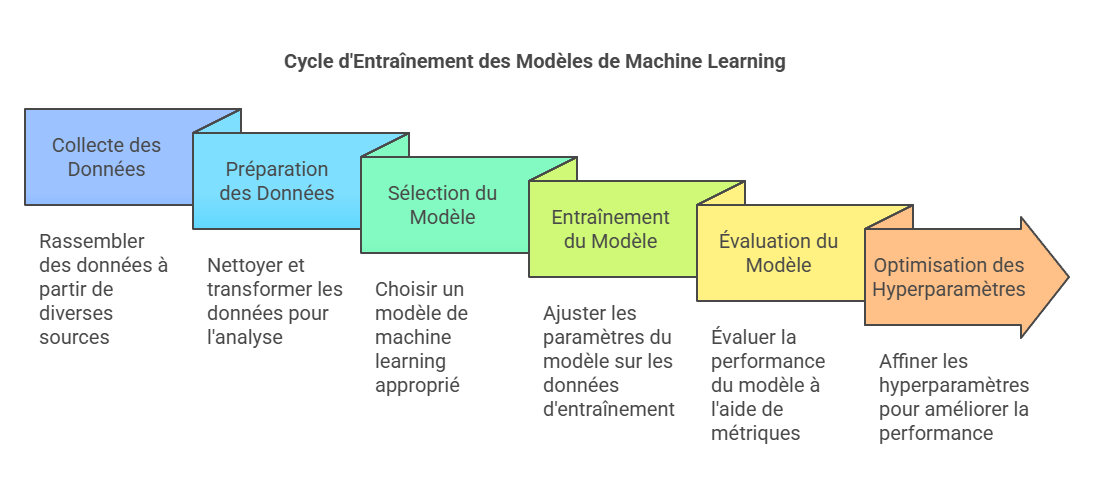
\includegraphics[width=\textwidth]{images/data_pipeline.png}
    \end{center}
    \begin{itemize}
        \item Processus itératif et structuré
        \item Chaque étape est cruciale pour le succès du projet
        \item Importance de la validation continue
        \item Nécessité d'une approche méthodique
    \end{itemize}
\end{frame}

% Collecte des données
\begin{frame}
    \frametitle{Étape 1 : Collecte des Données}
    \begin{columns}
        \column{0.5\textwidth}
        \includegraphics[width=\textwidth]{images/generated/data_collection.png}
        \column{0.5\textwidth}
        \begin{itemize}
            \item \textbf{Sources:}
            \begin{itemize}
                \item Bases de données publiques
                \item Images/vidéos collectées
                \item Données synthétiques générées
                \item Données externes annotées
            \end{itemize}
            \item \textbf{Considérations:}
            \begin{itemize}
                \item Qualité et quantité
                \item Distribution représentative
                \item Annotations adéquates
                \item Contraintes éthiques/légales
            \end{itemize}
        \end{itemize}
    \end{columns}
\end{frame}

% Traitement des données
\begin{frame}
    \frametitle{Étape 2 : Traitement des Données}
    \begin{center}
        \includegraphics[width=0.8\textwidth]{images/generated/data_processing.png}
    \end{center}
    \begin{itemize}
        \item \textbf{Nettoyage :} Suppression du bruit, correction des erreurs
        \item \textbf{Augmentation :} Génération de nouvelles données synthétiques
        \item \textbf{Feature Engineering :} Extraction des caractéristiques pertinentes
        \item \textbf{Normalisation :} Standardisation des données
    \end{itemize}
\end{frame}

% Exemple de traitement des données avec MNIST
\begin{frame}
    \frametitle{Exemple de Traitement des Données : MNIST}
    \begin{center}
        \includegraphics[width=\textwidth]{images/generated/data_processing_mnist.png}
    \end{center}
    \begin{itemize}
        \item \textbf{Data Augmentation :}
        \begin{itemize}
            \item Rotation : améliore la robustesse aux variations d'orientation
            \item Bruit : renforce la résistance aux perturbations
            \item Techniques additionnelles : translation, zoom, flou, retournement, changement de luminosité/contraste ...
        \end{itemize}
        \item \textbf{Feature Extraction :}
        \begin{itemize}
            \item Détection de contours : met en évidence les caractéristiques structurelles
            \item Autres techniques : filtres de Gabor, transformée de Fourier, wavelets ...
        \end{itemize}
    \end{itemize}
\end{frame}

% Entraînement et Validation
\begin{frame}
    \frametitle{Étape 3 : Entraînement et Validation}
    \begin{itemize}
        \item \textbf{Cycle d'entraînement :}
        \begin{itemize}
            \item Choix du modèle
            \item Définition de la loss
            \item Optimisation
            \item Validation
        \end{itemize}
    \end{itemize}
\end{frame}

% Déploiement et Production
\begin{frame}
    \frametitle{Étape 4 : Déploiement et Production}
    \begin{center}
        \includegraphics[width=0.9\textwidth]{images/generated/deployment.png}
    \end{center}
    \begin{itemize}
        \item \textbf{Validation finale :} Tests sur données réelles
        \item \textbf{Packaging :} Containerisation, API REST
        \item \textbf{Déploiement :} Cloud, Edge, On-premise
        \item \textbf{Monitoring :} 
        \begin{itemize}
            \item Surveillance des performances
            \item Détection de drift
            \item Maintenance continue
        \end{itemize}
    \end{itemize}
\end{frame}

% Transition vers la section sur la représentation des images
\begin{frame}
    \frametitle{Passons aux bases}
    \begin{center}
        \Huge{\textbf{Représentation Numérique des Images}}
    \end{center}
\end{frame}

% Section sur la représentation des images avec titre raccourci
\section{Représentation Numérique}

% Slide : Qu'est-ce qu'un pixel ?
\begin{frame}
    \frametitle{Qu'est-ce qu'un pixel ?}
    \begin{itemize}
        \item \textbf{Pixel} = Picture Element
        \item Plus petite unité d'une image numérique
        \item En couleur (RGB) :
        \begin{itemize}
            \item 3 valeurs : Rouge, Vert, Bleu
            \item Chaque valeur entre 0 et 255
            \item \(256^3 \approx 16.7\) millions de couleurs possibles
        \end{itemize}
        \item En niveaux de gris :
        \begin{itemize}
            \item 1 seule valeur entre 0 (noir) et 255 (blanc)
        \end{itemize}
    \end{itemize}
\end{frame}

% Slide : Exemple de pixel RGB
\begin{frame}
    \frametitle{Exemple de pixel RGB}
    \begin{center}
        \includegraphics[width=0.8\textwidth]{images/generated/rgb_pixel.png}
    \end{center}
    \begin{itemize}
        \item Un pixel RGB est un triplet de valeurs (R, G, B)
        \item Chaque canal a une valeur entre 0 et 255
        \item Combinaison = couleur spécifique
        \item Exemple : R=120, G=50, B=240 (teinte violette)
    \end{itemize}
\end{frame}

% Slide : De pixel à image
\begin{frame}
    \frametitle{De pixel à image : le plus simple exemple}
    \begin{center}
        \includegraphics[width=0.9\textwidth]{images/generated/two_pixels.png}
    \end{center}
    \begin{itemize}
        \item Une image est une matrice de pixels
        \item Le plus simple exemple : une image 1×2
        \item Dimensions de cette image minimale :
        \begin{itemize}
            \item Hauteur : 1 pixel
            \item Largeur : 2 pixels
            \item Profondeur : 3 canaux (RGB)
        \end{itemize}
    \end{itemize}
\end{frame}

% Slide : Exemple MNIST
\begin{frame}
    \frametitle{Exemple : Image MNIST}
    \begin{center}
        \includegraphics[width=0.9\textwidth]{images/generated/mnist_matrix.png}
    \end{center}
    \begin{itemize}
        \item MNIST : base de données de chiffres manuscrits
        \item Chaque image est une matrice 28×28 pixels (grayscale)
        \item Valeurs comprises entre 0 (noir) et 255 (blanc)
        \item Simple mais suffisant pour illustrer les concepts fondamentaux
    \end{itemize}
\end{frame}

% Slide : Image naturelle
\begin{frame}
    \frametitle{Image naturelle haute résolution}
    \begin{center}
        \includegraphics[width=0.95\textwidth]{images/generated/natural_image.png}
    \end{center}
    \begin{itemize}
        \item Images réelles : matrices beaucoup plus grandes
        \item Exemple : photo 4K = matrice 3840×2160×3
        \item \(\approx\) 24.9 millions de pixels !
    \end{itemize}
\end{frame}

% Slide : Vidéo et dimension temporelle
\begin{frame}
    \frametitle{Vidéo : L'ajout de la dimension temporelle}
    \begin{center}
        \includegraphics[width=0.95\textwidth]{images/generated/video_representation.png}
    \end{center}
    \begin{itemize}
        \item Vidéo = séquence d'images (frames) au cours du temps
        \item Tenseur 4D : Temps × Hauteur × Largeur × Canaux
        \item Exemple pour une vidéo HD 30fps, 10 secondes:
        \begin{itemize}
            \item 30 × 10 = 300 frames
            \item 300 × 1920 × 1080 × 3 = 1.86 milliards de valeurs !
        \end{itemize}
    \end{itemize}
\end{frame}

% Slide : Le défi de l'interprétation
\begin{frame}
    \frametitle{Le défi de l'interprétation}
    \begin{itemize}
        \item Pour l'ordinateur, une image n'est qu'une matrice de nombres
        \item Pas de notion intuitive de :
        \begin{itemize}
            \item Formes
            \item Objets
            \item Contexte
            \item Relations spatiales
        \end{itemize}
        \item \textbf{Challenge de la Vision par Ordinateur :}
        \begin{itemize}
            \item Extraire du sens de ces matrices de nombres
            \item Reproduire (et dépasser) la vision humaine
        \end{itemize}
    \end{itemize}
\end{frame}

% Transition vers les méthodes classiques
\begin{frame}
    \frametitle{Techniques traditionnelles}
    \begin{center}
        \Huge{\textbf{Méthodes Classiques}}
    \end{center}
\end{frame}

% Section sur les méthodes classiques avec titre raccourci
\section{Méthodes Classiques}

% Classification par seuillage de couleur
\begin{frame}
    \frametitle{Classification par Seuillage de Couleur}
    \begin{itemize}
        \item \textbf{Principe de la classification d'objets :}
        \begin{itemize}
            \item Identifier et catégoriser des objets dans une image
            \item Méthode simple : utilisation des caractéristiques de couleur
        \end{itemize}
        \item \textbf{Seuillage de couleur :}
        \begin{itemize}
            \item Définition de plages de valeurs pour chaque canal (R,G,B)
            \item Création d'un masque binaire
            \item Avantages : Simple, rapide
            \item Limites : Sensible aux variations de luminosité, angles, etc.
        \end{itemize}
    \end{itemize}
\end{frame}

\begin{frame}
    \frametitle{Exemple de Classification par Seuillage}
    \begin{center}
        \includegraphics[width=0.9\textwidth]{images/generated/color_thresholding.png}
    \end{center}
    \begin{itemize}
        \item \textbf{Principe:} Définir un seuil pour séparer les classes
        \item \textbf{Exemple:} Détection d'objets rouges
        \begin{itemize}
            \item Si R > 0.6 et G < 0.3 et B < 0.3 → objet rouge
            \item Sinon → fond
        \end{itemize}
    \end{itemize}
\end{frame}

% Soustraction d'images
\begin{frame}
    \frametitle{Détection de Changements par Soustraction d'Images}
    \begin{itemize}
        \item \textbf{Principe :}
        \begin{itemize}
            \item Comparaison de deux images similaires
            \item Soustraction pixel par pixel
            \item Détection des différences significatives
        \end{itemize}
        \item \textbf{Applications :}
        \begin{itemize}
            \item Détection de mouvement
            \item Surveillance vidéo
            \item Contrôle qualité industriel
        \end{itemize}
        \item \textbf{Avantages :}
        \begin{itemize}
            \item Simple à mettre en œuvre
            \item Efficace pour les changements nets
            \item Peu coûteux en calcul
        \end{itemize}
    \end{itemize}
\end{frame}

\begin{frame}
    \frametitle{Exemple Simple de Soustraction d'Images}
    \begin{center}
        \includegraphics[width=0.95\textwidth]{images/generated/image_subtraction.png}
    \end{center}
    \begin{itemize}
        \item \textbf{Principe:} Soustraire deux images pour détecter les différences
        \item \textbf{Exemple ci-dessus:}
        \begin{itemize}
            \item Image 1 : contient un rectangle
            \item Image 2 : contient un rectangle + un cercle
            \item Différence : fait ressortir uniquement le cercle
        \end{itemize}
        \item \textbf{Applications:} Détection de mouvement, surveillance, suivi d'objets
    \end{itemize}
\end{frame}

\begin{frame}
    \frametitle{Limites de la Soustraction Simple - Partie 1}
    \begin{center}
        \includegraphics[width=0.6\textwidth]{images/generated/real_video_subtraction.png}
    \end{center}
    \begin{itemize}
        \item Exemple avec vidéo réelle ($I_{1}$ et $I_{2}$ = deux frames)
        \item Différence brute $D(x,y) = |I_{2}(x,y) - I_{1}(x,y)|$
        \item Masque par seuillage : $M(x,y) = 1$ si $D(x,y) >$ seuil
        \item \textbf{Problèmes observés:} Bruit, trous, zones fragmentées
    \end{itemize}
\end{frame}

\begin{frame}
    \frametitle{Limites de la Soustraction Simple - Partie 2}
    \begin{itemize}
        \item \textbf{Masque de différence brute :}
        \begin{equation*}
            D(x,y) = |I_2(x,y) - I_1(x,y)|
        \end{equation*}
        \item \textbf{Masque binaire par seuillage :}
        \begin{equation*}
            M(x,y) = \begin{cases}
                1 & \text{si } D(x,y) > \text{seuil} \\
                0 & \text{sinon}
            \end{cases}
        \end{equation*}
        \item \textbf{Problèmes observés :}
        \begin{itemize}
            \item Bruit dans le masque de différence
            \item Faux positifs après seuillage
            \item Détections fragmentées
        \end{itemize}
        \item \textbf{Solution proposée :} Post-traitement par opérations morphologiques
    \end{itemize}
\end{frame}

% Opérations morphologiques
\begin{frame}
    \frametitle{Amélioration par Opérations Morphologiques}
    \begin{itemize}
        \item \textbf{Opérations morphologiques :}
        \begin{itemize}
            \item Transformation d'images basée sur la forme
            \item Utilisation d'un kernel
        \end{itemize}
        \item \textbf{Processus en deux étapes :}
        \begin{itemize}
            \item \textbf{1. Dilatation :} Expansion des objets et connexion des régions
            \begin{equation*}
                [D(M)]_{x,y} = \max_{(i,j) \in K} M_{x+i,y+j}
            \end{equation*}
            \item \textbf{2. Érosion :} Suppression du bruit et lissage des contours
            \begin{equation*}
                [E(M)]_{x,y} = \min_{(i,j) \in K} M_{x+i,y+j}
            \end{equation*}
        \end{itemize}
        où \(K\) est l'ensemble des coordonnées du kernel
    \end{itemize}
\end{frame}

\begin{frame}
    \frametitle{Application sur le Masque de Soustraction}
    \begin{center}
        \includegraphics[width=0.95\textwidth]{images/generated/morphological_operations.png}
    \end{center}
    \begin{itemize}
        \item \textbf{Dilatation:} Agrandit les régions blanches, comble les trous
        \item \textbf{Érosion:} Rétrécit les régions blanches, élimine le bruit
        \item \textbf{Combinaison:} Dilatation suivie d'érosion (fermeture)
        \item \textbf{Résultat:} Objets plus cohérents, moins bruités
    \end{itemize}
\end{frame}

\begin{frame}
    \frametitle{Détails des Opérations Morphologiques}
    \begin{itemize}
        \item \textbf{Propriétés :}
        \begin{itemize}
            \item Cette combinaison (D puis E) est appelée "fermeture morphologique"
            \item Fermeture : comble les trous et connecte les régions proches
            \item Ouverture : élimine les petits objets et le bruit (E puis D)
        \end{itemize}
    \end{itemize}
\end{frame}

% Transition vers les convolutions
\begin{frame}
    \frametitle{Opération fondamentale}
    \begin{center}
        \Huge{\textbf{Convolutions}}
    \end{center}
\end{frame}

% Section sur les convolutions avec titre raccourci
\section{Convolutions}

% Introduction aux convolutions
\begin{frame}
    \frametitle{La Convolution : Une Opération Fondamentale}
    \begin{itemize}
        \item \textbf{Définition :} Opération mathématique combinant deux fonctions
        \item En vision par ordinateur : 
        \begin{itemize}
            \item Combine une image avec un filtre (kernel)
            \item Extrait des caractéristiques spécifiques
            \item Base des réseaux de neurones convolutifs
        \end{itemize}
        \item \textbf{Formule mathématique en 2D :}
        \[ (f * k)(x,y) = \sum_{i=-a}^a \sum_{j=-b}^b f(x-i,y-j)k(i,j) \]
        où \(f\) est l'image et \(k\) est le kernel
    \end{itemize}
\end{frame}

% Exemple concret de convolution
\begin{frame}
    \frametitle{Exemple de Convolution 2D}
    \begin{center}
        \includegraphics[width=\textwidth]{images/generated/convolution_operation.png}
    \end{center}
    \begin{itemize}
        \item Convolution = opération fondamentale en CV
        \item Exemple ci-dessus avec filtre vertical simple
        \item Chaque position : somme pondérée du voisinage et du noyau
        \item Résultat : détection des transitions verticales
    \end{itemize}
\end{frame}

% Animation de convolution
\begin{frame}
    \frametitle{Animation du Processus de Convolution}
    \begin{center}
        %\animategraphics[loop,controls,width=0.8\textwidth]{5}{images/generated/gif/convolution_animation}{000}{312}
        \includegraphics[width=0.8\textwidth]{images/generated/gif/convolution_animation000.png}
    \end{center}
    \begin{itemize}
        \item Le noyau glisse sur l'image d'entrée
        \item À chaque position : multiplication élément par élément et somme
        \item L'exemple utilise un filtre de Sobel vertical (détecte les bords verticaux)
        \item Résultat : carte d'activation des contours verticaux
    \end{itemize}
\end{frame}

% Paramètres de convolution
\begin{frame}
    \frametitle{Paramètres d'une Convolution}
    \begin{itemize}
        \item \textbf{Taille du noyau:} contrôle la zone d'influence (3×3, 5×5, 7×7...)
        \item \textbf{Padding:} Préservation ou non des dimensions de l'image
        \item \textbf{Stride:} Pas de déplacement du noyau (généralement 1 ou 2)
        \item \textbf{Dilation:} Espacement entre les éléments du noyau
    \end{itemize}
    \begin{center}
        \includegraphics[width=0.8\textwidth]{images/generated/convolution_parameters.png}
    \end{center}
\end{frame}

% Filtres de convolution courants
\begin{frame}
    \frametitle{Filtres de Convolution Classiques}
    \begin{columns}
        \begin{column}{0.6\textwidth}
            \includegraphics[width=\textwidth]{images/generated/convolution_filters.png}
        \end{column}
        \begin{column}{0.4\textwidth}
            \textbf{Kernels utilisés :}
            \vspace{0.3cm}
            
            \textbf{Sobel vertical :}
            \[
            \begin{smallmatrix}
            -1 & 0 & 1 \\
            -2 & 0 & 2 \\
            -1 & 0 & 1
            \end{smallmatrix}
            \]
            
            \textbf{Sobel horizontal :}
            \[
            \begin{smallmatrix}
            -1 & -2 & -1 \\
            0 & 0 & 0 \\
            1 & 2 & 1
            \end{smallmatrix}
            \]
            
            \textbf{Flou (moyenne) :}
            \[
            \begin{smallmatrix}
                \frac{1}{9} & \frac{1}{9} & \frac{1}{9} \\
                \frac{1}{9} & \frac{1}{9} & \frac{1}{9} \\
                \frac{1}{9} & \frac{1}{9} & \frac{1}{9}
            \end{smallmatrix}
            \]
        \end{column}
    \end{columns}
\end{frame}

% Transition vers les CNN
\begin{frame}
    \frametitle{Apprentissage des convolutions}
    \begin{center}
        \Huge{\textbf{Réseaux CNN}}
    \end{center}
\end{frame}

% Section sur les CNN avec titre raccourci
\section{Réseaux CNN}

% Introduction aux CNN
\begin{frame}
    \frametitle{Des Filtres Fixes aux Filtres Appris}
    \begin{itemize}
        \item \textbf{Limitation des filtres prédéfinis :}
        \begin{itemize}
            \item Choix manuel des filtres
            \item Pas d'adaptation aux données
            \item Nombre limité de features extraites
        \end{itemize}
        \item \textbf{Solution : Apprentissage automatique des filtres}
        \begin{itemize}
            \item Les filtres deviennent des paramètres à optimiser
            \item Adaptation aux caractéristiques importantes des données
            \item Minimisation d'une fonction de perte
        \end{itemize}
    \end{itemize}
\end{frame}

% Exemple simple de CNN
\begin{frame}
    \frametitle{Exemple Simple : Détection de Lignes Verticales}
    \begin{center}
        \includegraphics[width=0.8\textwidth]{images/generated/simple_cnn_vertical.png}
    \end{center}
    \begin{itemize}
        \item \textbf{Observation :} Le CNN apprend des filtres adaptés aux tâches
        \item \textbf{Exemple :} Filtre appris pour la détection de lignes verticales
        \item \textbf{Résultat :} Activation forte pour les lignes verticales, faible pour horizontales
    \end{itemize}
\end{frame}

% CNN plus profond
\begin{frame}
    \frametitle{Vers des Architectures Plus Profondes}
    \begin{center}
        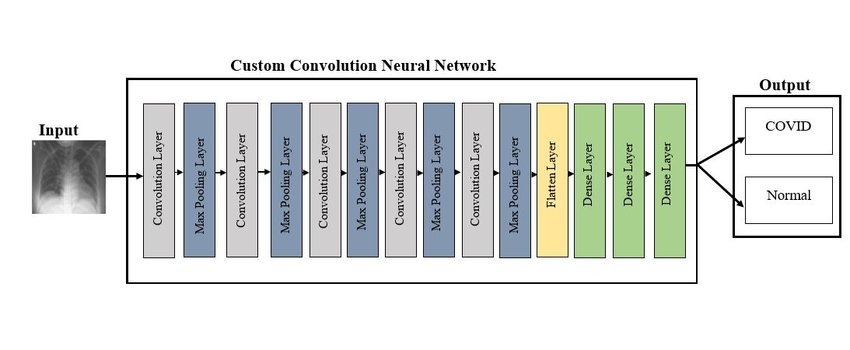
\includegraphics[width=0.95\textwidth]{images/CNN_example.png}
    \end{center}
    \begin{itemize}
        \item \textbf{Avantages de la profondeur :}
        \begin{itemize}
            \item Extraction de caractéristiques plus complexes
            \item Hiérarchie de features (des simples aux complexes)
            \item Meilleure capacité de généralisation
        \end{itemize}
    \end{itemize}
\end{frame}

% Pooling
\begin{frame}
    \frametitle{Le Rôle du Pooling}
    \begin{itemize}
        \item \textbf{Objectifs du pooling :}
        \begin{itemize}
            \item Réduction de la dimension spatiale
            \item Invariance aux petites translations
            \item Réduction du nombre de paramètres
        \end{itemize}
        \item \textbf{Types de pooling :}
        \begin{itemize}
            \item Max pooling : valeur maximale de la région
            \item Average pooling : moyenne de la région
        \end{itemize}
        \item \textbf{Paramètres :}
        \begin{itemize}
            \item Taille de la fenêtre (généralement 2×2)
            \item Stride (généralement égal à la taille)
        \end{itemize}
    \end{itemize}
\end{frame}

% ResNet
\begin{frame}
    \frametitle{ResNet : L'Innovation des Skip Connections}
    \begin{columns}
        \column{0.6\textwidth}
        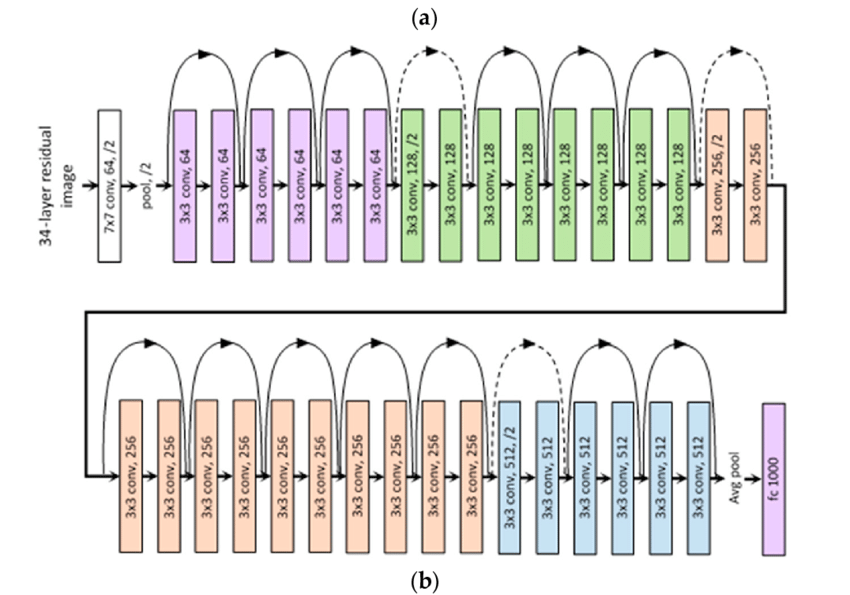
\includegraphics[width=\textwidth, angle=-90]{images/resnet.png}
        
        \column{0.4\textwidth}
        \textbf{Avantages :}
        \begin{itemize}
            \item Facilite l'entraînement des réseaux profonds
            \item Atténue le problème de la disparition du gradient
            \item Permet l'apprentissage résiduel
        \end{itemize}
    \end{columns}
\end{frame}

\begin{frame}
    \frametitle{Pourquoi les Skip Connections ?}
    \begin{itemize}
        \item \textbf{Problème des réseaux profonds :}
        \begin{itemize}
            \item Difficulté d'apprentissage
            \item Dégradation des performances
        \end{itemize}
        \item \textbf{Solution ResNet :}
        \begin{itemize}
            \item \(F(x) + x\) au lieu de \(F(x)\)
            \item Si \(F(x) = 0\), on préserve l'identité
            \item Apprentissage des résidus
        \end{itemize}
        \item \textbf{Impact :}
        \begin{itemize}
            \item Entraînement plus stable
            \item Convergence plus rapide
            \item Meilleures performances
        \end{itemize}
    \end{itemize}
\end{frame}


% Slide : GitHub et Questions
\begin{frame}
    \frametitle{Ressources et Questions}
    \begin{center}
        \textbf{\large{Retrouvez tous les supports de cours sur GitHub: }}
        
        \vspace{0.5cm}
        
\includegraphics[width=0.2\textwidth]{images/github.png}
                \begin{tcolorbox}[colback=black!5!white,colframe=black!75!white,width=0.8\textwidth]
            \centering
            \large{\href{https://github.com/fvalade/Computer-vision-Course-Materials}{\textcolor{blue}{github.com/fvalade/Computer-vision-Course-Materials}}}
        \end{tcolorbox}
        
        \huge{\textbf{Des questions ?}}
    \end{center}
\end{frame}

\end{document}
